%%%%%%%%%%%%%%%%%%%%%%%%%%%%%%%%%%%%%%%%%%%%%%%%%%%%%%%%%%%%%%%%%%%%%%%%%%%%%%%%
% \documentclass[12pt,papel,twoside]{unrnpfi}
\documentclass[12pt,screen,twoside,pagebackref]{unrnpfi}
% \documentclass[12pt,papel,singlespace,oneside]{unrnpfi}
% \documentclass[12pt,papel,preprint,singlespace,oneside]{unrnpfi}


%%%%%%%%%%%%%%%%%%%%% Paquetes extra %%%%%%%%%%%%%%%%%%%%%%%%%%%%%%%%%%%%%%%%%%%
% Por conveniencia: aqu\'{\i} puede cargar todos los paquetes y definir los comandos 
% que necesite
\usepackage{unrnextra}
%%%%%%%%%%%%%%%%%%%%%%%%%%%%%%%%%%%%%%%%%%%%%%%%%%%%%%%%%%%%%%%%%%%%%%%%%%
%%%%%%%%%
\palabrasclave{Formato de PFI, Plantilla, Universidad Nacional de Río Negro}
\keywords{PFI format, Templates, Universidad Nacional de Río Negro}

%%%%%%%%%%%%%%%%%%%%%%%%%%%%%%%%%%%%%%%%%%%%%%%%%%%%%%%%%%%%%%%%%%%%%%%%%%%%%%%%
%\titlepagefalse % Si no quiere compilar la portada descomente esta linea
%\includeonly{apendices} % Compilar s\'{o}lo estos archivos 
\graphicspath{{figs/}} % Lugar donde encontrar las figuras generales (se puede poner uno en cada cap{\'{\i}}tulo)
%%%%%%%%%%%%%%%%%%%%%%%%%%%%%%%%%%%%%%%%%%%%%%%%%%%%%%%%%%%%%%%%%%%%%%%%%%%%%%%%


\begin{document}

% Dentro del environment 'preliminary' va:
% la dedicatoria, resumen, abstract, indices

\begin{preliminary}

% Escriba su dedicatoria
\dedicatoria{
A mi familia\\
A mis amigos\\
A todos los que me conocen\\
A toda esa otra gente que no
}

%%% \'{I}ndices %%%%

\begin{abreviaturas}
UNRN: Universidad Nacional de Río Negro.\\
PFI: Proyecto Final Integrador.
\end{abreviaturas}

\tableofcontents                %\'{I}ndice

\listoffigures                  %Figuras

\listoftables                   %Tablas

\begin{resumen}%
Este es el resumen en castellano.\\
El PFI debe reflejar el trabajo desarrollado, mostrando la metodolog\'{\i}a utilizada, los resultados obtenidos y las conclusiones que pueden inferirse de dichos resultados.
\end{resumen}

\begin{abstract}%
This is the title in English:\\
The thesis must reflect the work of the student, including the chosen methodology, the results and the conclusions that those results allow us to draw.
\end{abstract}


%%% Local Variables: 
%%% mode: latex
%%% TeX-master: "main"
%%% End: 


\end{preliminary}


% Podemos usar cualquiera de los dos comandos: \input o \include para incluir el texto
\chapter{Uso del estilo provisto}
\chapterquote{Hablaban siempre de dinero y planeaban asaltar un banco}{Domingo Cavallo, 2001}

\section{Opciones que acepta el estilo}
\label{S:opciones-que-acepta}

\subsection*{Espaciado}
El interlineado que se utiliza en el cuerpo de la tesis es de un espacio y medio. Esto se puede cambiar usando una de las opciones
\begin{itemize}
\item Un espacio y medio(\textbf{default})
\item un s\'{o}lo espacio (\verb|\documentclass[12pt,singlespacing]{unrnpfi}|)
\item doble espacio (\verb|\documentclass[12pt,doublespacing]{unrnpfi}|)
\end{itemize}

\subsection*{Formato de la p\'{a}gina}
El formato de la p\'{a}gina puede ser
\begin{itemize}
\item final Es el recomendado(\textbf{default})
\item borrador (\verb|\documentclass[12pt,preprint]{unrnpfi}|)\\ Es un formato con m\'{a}rgenes m\'{a}s chicos, \'{u}til para realizar correcciones en borradores 
\end{itemize}

\subsection*{Doble faz}
\label{S:doble-faz}

\begin{itemize}
\item \verb|\oneside| Los m\'{a}rgenes son iguales para todas las p\'{a}ginas
\item \verb|\twoside| P\'{a}ginas izquierdas y derechas son diferentes
\end{itemize}

\subsection*{Soporte f\'{\i}sico}

El estilo tiene una opci\'{o}n para soporte en papel y en pantalla:
\begin{itemize}
\item En papel (\verb|\documentclass[12pt,paper]{ibtesis}|) (\textbf{default})
\item En pantalla (archivo pdf) (\verb|\documentclass[12pt,screen]{ibtesis}|)\\
Incluye links y algunos colores en el texto
\end{itemize}

\subsection*{Otras opciones}
\label{S:otras-opciones}
Otras opciones con las que se cargue el estilo se pasan directamente a los estilos usados. Por ejemplo si usamos:\\
\verb|\documentclass[11pt,screen,oneside,preprint,draft,pagebackref]{unrnpfi}|\\
producir\'{a} un documento con letra de menor tama\~{n}o (11pt), no se procesar\'{a}n los gr\'{a}ficos (draft) para una mayor velocidad, se producir\'{a}n links en el archivo pdf con la caracter\'{\i}stica adicional que las referencias tendr\'{a}n un link al lugar donde fueron citadas ya que la opci\'{o}n \verb|pagebackref| se pasa al paquete \verb|\hyperref|.

\section{Par\'{a}metros convenientes}
\label{S:param-conv}

Se han definido tres longitudes que pueden servir para dar un ancho uniforme a todas las figuras.
Estas longitudes se han definido s\'{o}lo por conveniencia. 

Los valores que se le han dado son:
\begin{itemize}
\item \verb|\imsize= 0.7\textwidth|
\item \verb|\imsizeS= 0.5\textwidth|
\item \verb|\imsizeL= 0.9\textwidth|
\end{itemize}

Si se quieren modificar, puede hacerse usando el comando \verb|\setlength|, por ejemplo:
\begin{itemize}
\item \verb|\setlength{\imsizeL}{0.85\textwidth}|
\item \verb|\setlength{\imsize}{3.6in}|
\item \verb|\setlength{\imsizeS}{8.6cm}|
\end{itemize}

%%% Local Variables: 
%%% mode: latex
%%% TeX-master: "main"
%%% End: 

\chapter{Algunos ejemplos y usos}
\graphicspath{{figs/}}

\chapterquote{Que mira bobo}{Lionel Messi, 2023}

\label{C:algunos-ejemplos-y-usos}


%%%%%%%%%%%%%%%%%%%%%%%%%%%%%%%%%%%%%%%%%%%%%%%%%%%%%%%%%%%%%%%%%%%%%%%%
\section{Uso de listas}
\label{S:uso-de-listas}

El problema de la medida se puede describir informalmente del siguiente modo \cite{Bohr1913PMp10}

\begin{enumerate}
    \item hola 1.
        \begin{itemize}
          \item Item 1
          \item Item 2
        \end{itemize}
    \item hola 2.
        \begin{description}
            \item[Item 1:] Descripcion Item 1
            \item[Item 2:] Descripcion Item 2
        \end{description}
    \item hola 3 (ver notas a continuaci\'{o}n) \cite{Bohm1952PRp166,Bohm1952PRp180}:
        \begin{enumerate}
        \item hola a.
        \item hola b.
        \item hola c.
        \end{enumerate}
        
\end{enumerate}


\section{Uso de Imagenes}
\label{S:uso-de-imagenes}
Como incluir una imagen:\\
\begin{figure}[!ht]
\centering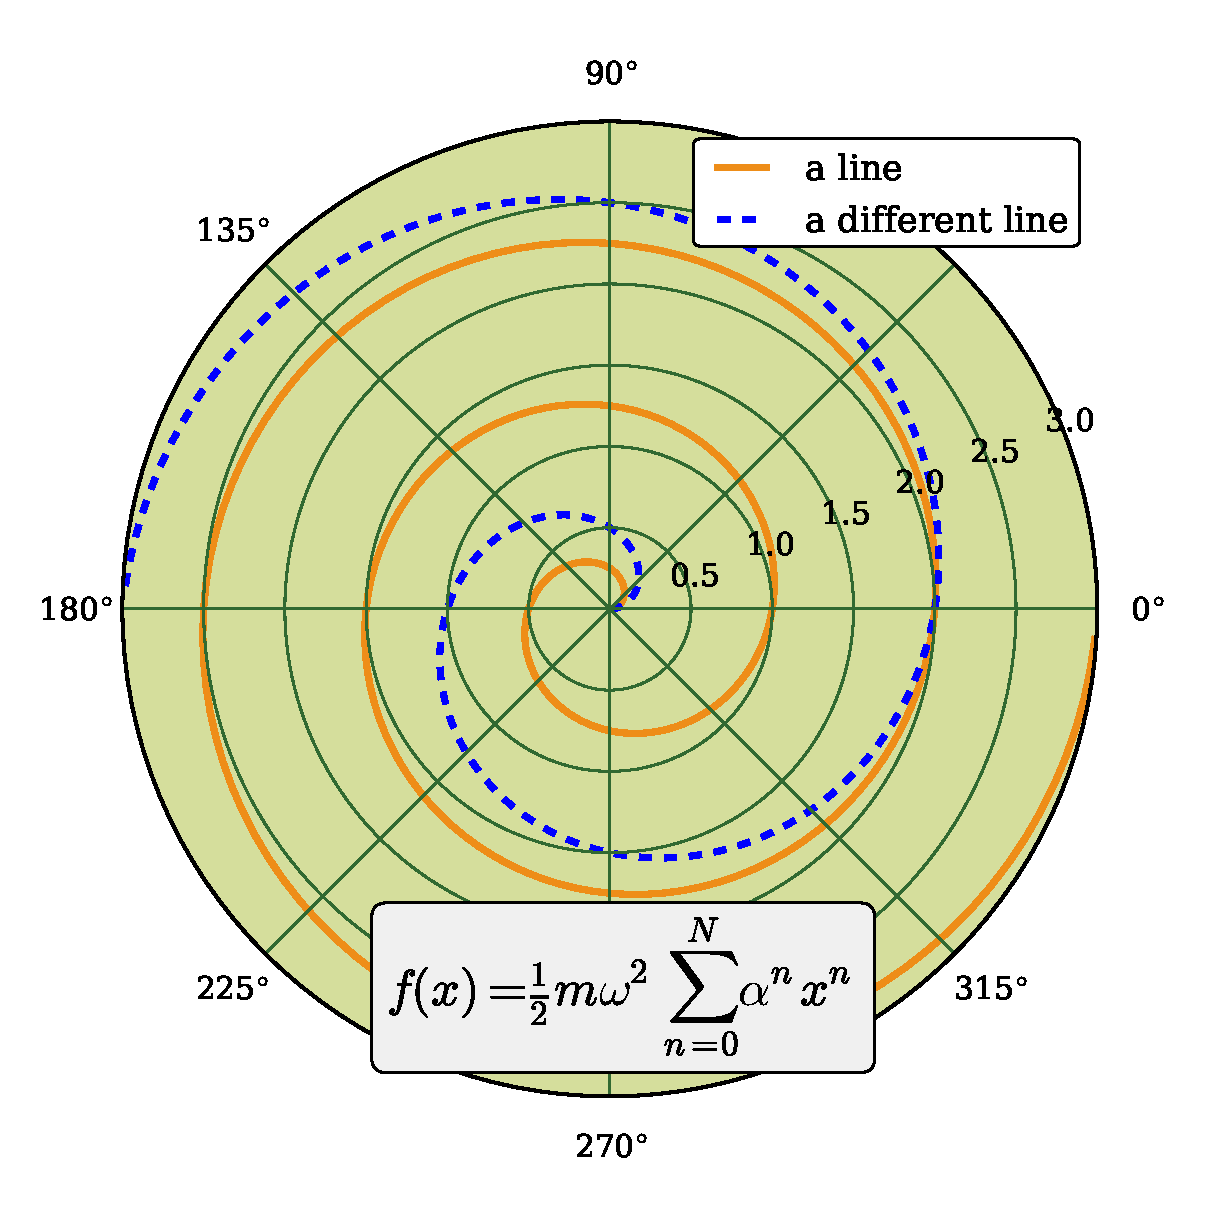
\includegraphics[width=\imsize]{cap2_f1}
\caption[La figura muestra algunas curvas m\'{a}s o menos lindas]{La figura muestra algunas curvas m\'{a}s o menos lindas. El gr\'{a}fico est\'{a} en coordenadas porlares como se muestra en la ref.~\protect{\cite{Hunter07CSE}}}
\end{figure}

\section{Uso de Ecucaciones}
\label{S:uso-de-ecuaciones}
En la primera ecuaci\'{o}n
\begin{equation}
\phi_{1}(z)=A_{1}e^{ik_{1}z}+B_{1}e^{-ik_{1}z}.
\end{equation}

En la segunda ecuaci\'{o}n:
\begin{equation}
\phi_{2}(z)=A_{2}e^{ik_{2}z}+B_{2}e^{-ik_{2}z}.
\end{equation}

\section{Uso de código}
\label{S:uso-de-codigo}

Podemos agregar lineas de código\footnote{\url{https://www.overleaf.com/learn/latex/Code_Highlighting_with_minted}}:
\begin{center}
    \begin{minted}{python}
        for n in range(10):
        if n%2:
        print n
    \end{minted}
\end{center}

También podemos importar código:
\inputminted{python}{cods/holamundo.py}

\section{Uso de circuitikz}
\label{S:uso-de-circuitikz}
Para dibujar circuitos podemos usar Ciruitikz\footnote{\url{https://www.overleaf.com/learn/latex/CircuiTikz_package}}

\begin{figure}[!ht]
    \centering
    \shorthandoff{<>}
    	\begin{circuitikz}[european voltages] \draw
    		(0,0) to [short, *-] (6,0)
                to [V, l_=$\mathrm{j}{\omega}_m \underline{\psi}^s_R$] (6,2) 
                to [R, l_=$R_R$] (6,4) 
                to [short, i_=$\underline{i}^s_R$] (5,4) 
                (0,0) to [open, v^>=$\underline{u}^s_s$] (0,4) 
                to [short, *- ,i=$\underline{i}^s_s$] (1,4) 
                to [R, l=$R_s$] (3,4)
                to [L, l=$L_{\sigma}$] (5,4) 
                to [short, i_=$\underline{i}^s_M$] (5,3) 
                to [L, l_=$L_M$] (5,0);
    	\end{circuitikz}
    \shorthandon{<>}
    \caption{Hola este es el caption del circuito\label{f:ModeloCircuito}}
\end{figure}

%%% Local Variables: 
%%% mode: latex
%%% TeX-master: "main"
%%% End: 

hola mundo

\appendix
\chapter{Ejemplo de ap\'{e}ndice: El problema de la medida}\label{C:ap1}
\chapterquote{Que miseria che, tres empanadas}{Brandoni, 2018}
\graphicspath{{figs/}}
%%%%%%%%%%%%%%%%%%%%%%%%%%%%%%%%%%%%%%%%%%%%%%%%%%%%%%%%%%%%%%%%%%%%%%%%
Una figura en el apendice se ve así,
\begin{figure}[ht]
\centering{}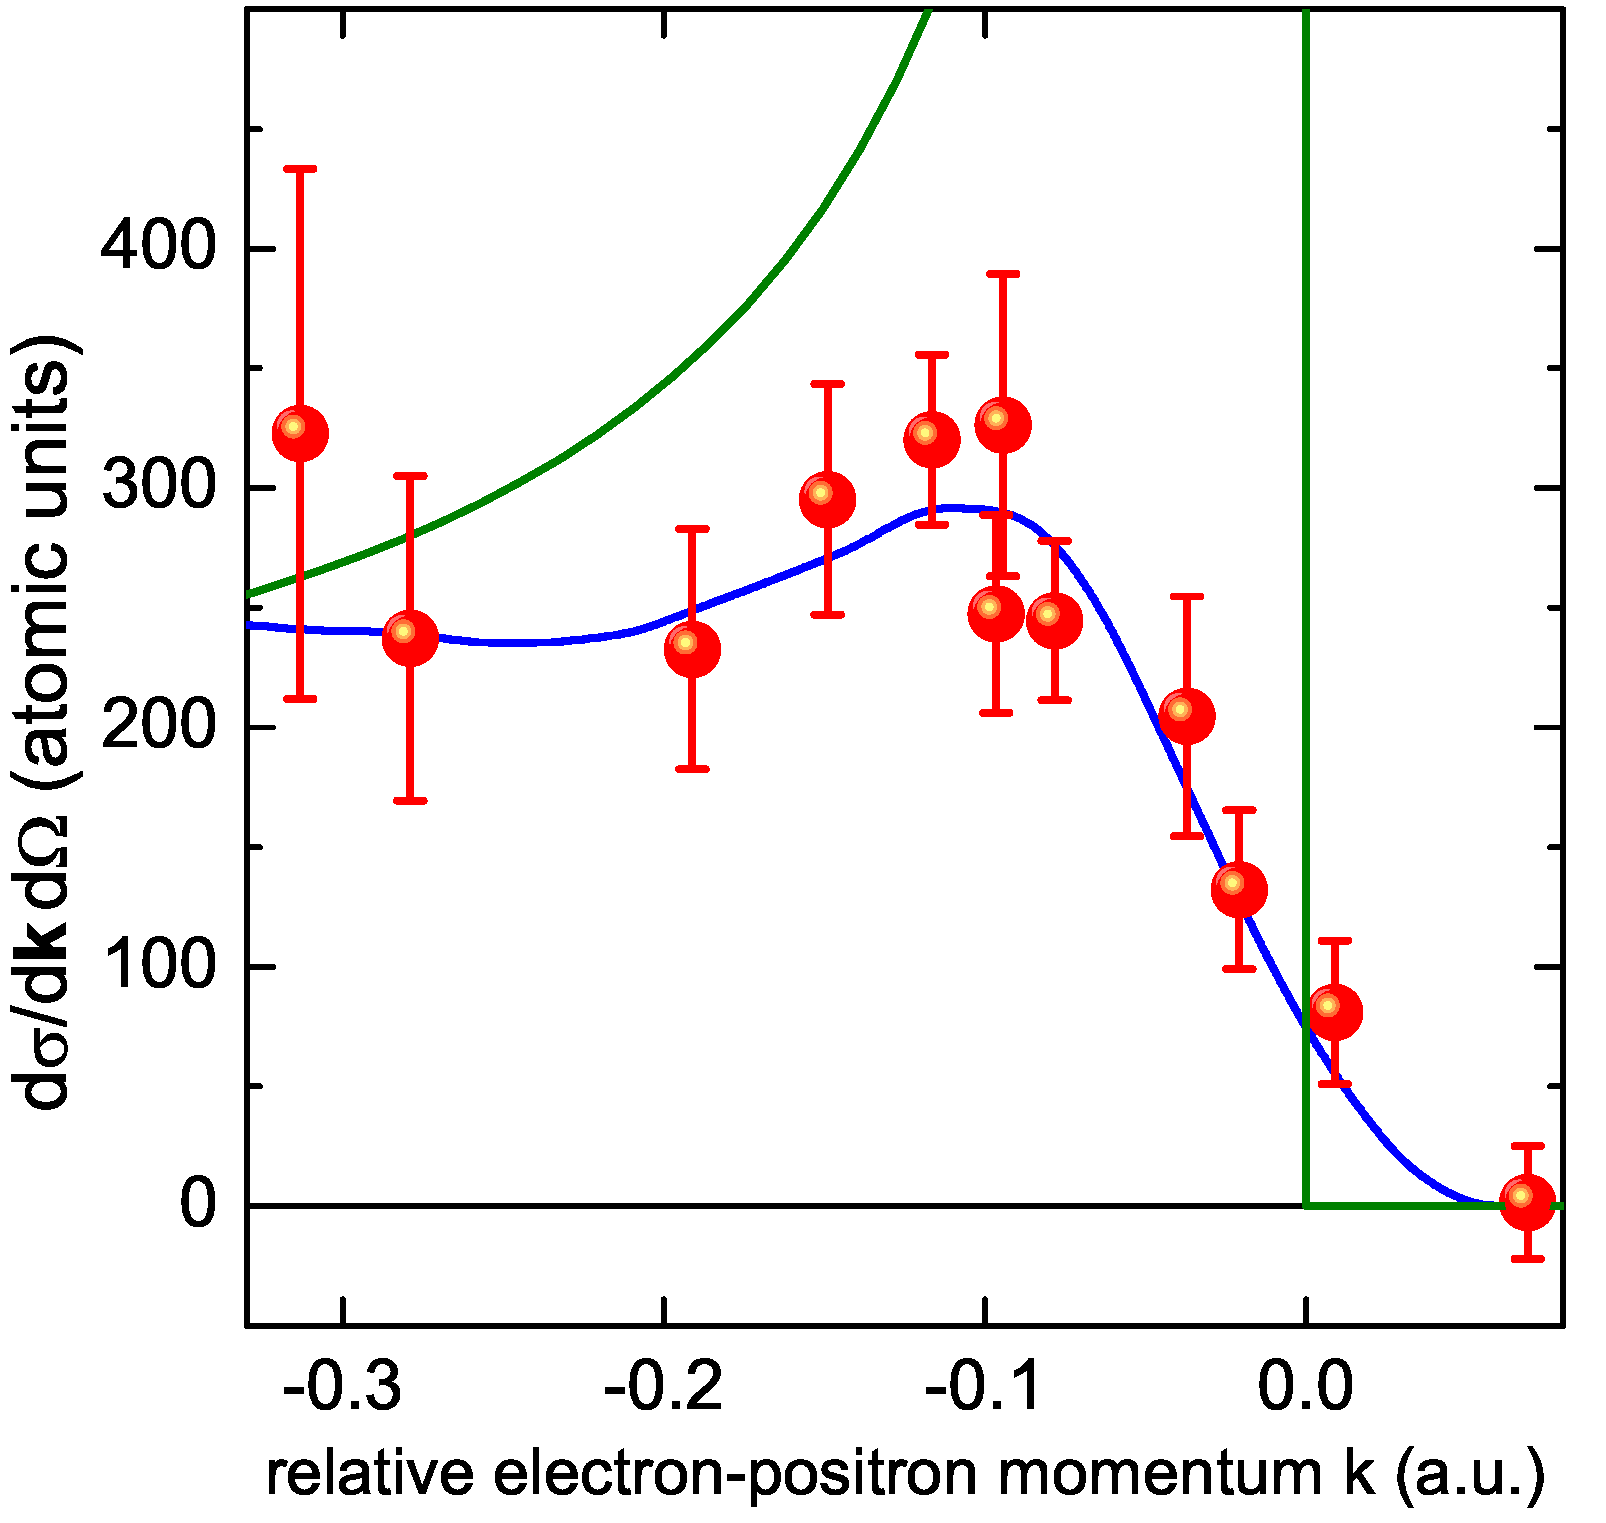
\includegraphics[width=\imsize]{ap1_f1}
\caption{Una figura con algunos puntos experimentales y curva de datos te\'{o}ricos\label{f:figura1}}  
\end{figure}

%%% Local Variables: 
%%% mode: latex
%%% TeX-master: "main"
%%% End: 


\begin{biblio}
\bibliography{mibib}
\end{biblio}

\begin{postliminary}

\begin{seccion}{Agradecimientos}
A todos los que se lo merecen, por merecerlo.
\end{seccion}

\end{postliminary}

\end{document}

